\documentclass[12pt,oneside,english]{book}
\usepackage{babel}
\usepackage[utf8]{inputenc}
\usepackage[T1]{fontenc}
\usepackage{color}
\definecolor{marron}{RGB}{60,30,10}
\definecolor{darkblue}{RGB}{0,0,80}
\definecolor{lightblue}{RGB}{80,80,80}
\definecolor{darkgreen}{RGB}{0,80,0}
\definecolor{darkgray}{RGB}{0,80,0}
\definecolor{darkred}{RGB}{80,0,0}
\definecolor{shadecolor}{rgb}{0.97,0.97,0.97}
\usepackage{graphicx}
\usepackage{wallpaper}
\usepackage{wrapfig,booktabs}

\usepackage{fancyhdr}
\usepackage{lettrine}
\input Acorn.fd

\renewcommand{\familydefault}{pplj} 
\usepackage[
final,
stretch=10,
protrusion=true,
tracking=true,
spacing=on,
kerning=on,
expansion=true]{microtype}

%\setlength{\parskip}{1.5ex plus 0.2ex minus 0.2ex}


\usepackage{fourier-orns}
\newcommand{\dash}{\vspace{2em}\noindent \textcolor{darkgray}{\hrulefill~ \raisebox{-2.5pt}[10pt][10pt]{\leafright \decofourleft \decothreeleft  \aldineright \decotwo \floweroneleft \decoone   \floweroneright \decotwo \aldineleft\decothreeright \decofourright \leafleft} ~  \hrulefill \\ \vspace{2em}}}
\newcommand{\rdash}{\noindent \textcolor{darkgray}{ \raisebox{-1.9pt}[10pt][10pt]{\leafright} \hrulefill \raisebox{-1.9pt}[10pt][10pt]{\leafright \decofourleft \decothreeleft  \aldineright \decotwo \floweroneleft \decoone}}}
\newcommand{\ldash}{\textcolor{darkgray}{\raisebox{-1.9pt}[10pt][10pt]{\decoone \floweroneright \decotwo \aldineleft \decothreeright \decofourright \leafleft} \hrulefill \raisebox{-1.9pt}[10pt][10pt]{\leafleft}}}

\fancyhf{}

\renewcommand{\chaptermark}[1]{\markboth{#1}{}}
\renewcommand{\sectionmark}[1]{\markright{#1}}

\newcommand{\estcab}[1]{\itshape\textcolor{marron}{\nouppercase #1}}

\fancyhead[LO]{\estcab{\rightmark}} 
\fancyhead[RO]{\estcab{\leftmark}}
\fancyhead[RO]{\bf\nouppercase{ \leftmark}}
\fancyfoot[RO]{ \leafNE  ~~ \bf \thepage}

\newenvironment{Section}[1]
{\section{\vspace{0ex}#1}}
{\vspace{12pt}\centering ------- \decofourleft\decofourright ------- \par}

\usepackage{lipsum}
\setlength{\parindent}{1em} % Sangría española
\pagestyle{fancy}

\renewcommand{\footnoterule}{\noindent\textcolor{marron}{\decosix \raisebox{2.9pt}{\line(1,0){100}} \lefthand} \vspace{.5em} }
\usepackage[hang,splitrule]{footmisc}
\addtolength{\footskip}{0.5cm}
\setlength{\footnotemargin}{0.3cm}
\setlength{\footnotesep}{0.4cm} 

\usepackage{chngcntr}
\counterwithout{figure}{chapter}
\counterwithout{table}{chapter}

\usepackage{kotex}
\usepackage{amsthm} 
\usepackage{amsmath} 
\usepackage{amsfonts}
\usepackage{enumerate} 
\usepackage{cite}
\usepackage{graphics} 
\usepackage{graphicx,lscape} 
\usepackage{subcaption}
\usepackage{algpseudocode}
\usepackage{algorithm}
\usepackage{titlesec}
\usepackage{cite, url}
\usepackage{amssymb}

\def\ck{\paragraph{\Large$\bullet$}\Large}
\def\goal{\paragraph{\Large(목표)}\Large}
\def\observe{\paragraph{\Large(관찰)}\Large}
\def\assume{\paragraph{\Large(가정)}\Large}
\def\summary{\paragraph{\Large(요약)}\Large}
\def\EX{\paragraph{\Large(예제)}\Large}
\def\guess{\paragraph{\Large(추측)}\Large}
\def\thus{\paragraph{\Large(결론)}\Large}
\def\prob{\paragraph{\Large(문제)}\Large}
\def\sol{\paragraph{\Large(해결)}\Large}
\def\dfn{\paragraph{\Large(정의)}\Large}
\def\thm{\paragraph{\Large(정리)}\Large}
\def\lem{\paragraph{\Large(레마)}\Large}
\def\promise{\paragraph{\Large(약속)}\Large}
\def\property{\paragraph{\Large(특징)}\Large}
\def\fl{\paragraph{\Large(느낌)}\Large}
\def\memo{\paragraph{\Large(암기)}\Large}
\def\note{\paragraph{\Large\textit{\underline{note:}}}\Large}
\def\ex{\paragraph{\Large\textit{example:}}\Large}


\def\one{\paragraph{\Large(1)}\Large}
\def\two{\paragraph{\Large(2)}\Large}
\def\three{\paragraph{\Large(3)}\Large}
\def\four{\paragraph{\Large(4)}\Large}
\def\five{\paragraph{\Large(5)}\Large}
\def\six{\paragraph{\Large(6)}\Large}
\def\seven{\paragraph{\Large(7)}\Large}
\def\eight{\paragraph{\Large(8)}\Large}
\def\nine{\paragraph{\Large(9)}\Large}
\def\ten{\paragraph{\Large(10)}\Large}

\newcommand{\bld}[1]{\mbox{\boldmath $#1$}}

\DeclareMathOperator*{\argmin}{arg\,min} %\usepackage{amsmath}를 써야지 정의가능함. 
\DeclareMathOperator*{\argmax}{arg\,max} %\usepackage{amsmath}를 써야지 정의가능함. 

\usepackage{titlesec}
\titleformat*{\section}{\huge\bfseries}
\titleformat*{\subsection}{\huge\bfseries}
\titleformat*{\subsubsection}{\huge\bfseries}
\titleformat*{\paragraph}{\huge\bfseries}
\titleformat*{\subparagraph}{\huge\bfseries}


\titleclass{\part}{top}
\titleformat{\part}[display]
  {\normalfont\huge\bfseries}{\centering\partname\ \thepart}{20pt}{\Huge\centering}
\titlespacing*{\part}{0pt}{50pt}{40pt}
\titleclass{\chapter}{straight}
\titleformat{\chapter}[display]
  {\normalfont\huge\bfseries}{\chaptertitlename\ \thechapter}{20pt}{\Huge}
\titlespacing*{\chapter} {0pt}{50pt}{40pt}

\newcommand*\initfamily{\usefont{U}{Acorn}{xl}{n}}
\usepackage[left=10px,right=10px,top=10px,bottom=10px,paperwidth=8in,paperheight=115in]{geometry}

\usepackage{geometry}
\geometry{
tmargin=3cm, 
bmargin=3cm, 
lmargin=1cm, 
rmargin=1cm,
headheight=1.5cm,
headsep=0.8cm,
footskip=0.5cm}


% Insert R code to LaTeX.
\usepackage[svgnames]{xcolor}
\usepackage{listings}

\lstset{
language=R,
basicstyle=\scriptsize\ttfamily,
commentstyle=\ttfamily\color{DarkGreen},
numbers=left,
numberstyle=\ttfamily\color{gray}\footnotesize,
stepnumber=1,
numbersep=5pt,
backgroundcolor=\color{white},
showspaces=false,
showstringspaces=false,
showtabs=false,
frame=single,
tabsize=2,
captionpos=b,
breaklines=true,
breakatwhitespace=false,
%title=\lstname,
escapeinside={},
keywordstyle=\color{blue},
otherkeywords={!,!=,~,\&,\%/\%,\%\%,<-,<<-,/,0,1,2,3,4,5,6,7,8,9},
deletekeywords={data,mean,sd,stem,rnorm,density,range,rgb,plot,panel,polygon,col,legend,grid,matrix,set,ncol,rbind,cbind,colnames,D_hat,max,old,sample,D,sqrt,hat,sum,_,solve,nrow,par,summary,table,options,c,frame,length,as,character},
}


\begin{document}
\chapter{시계열 12주차 강의내용}
\section{시계열의 추세}

\ck 적당한 과정에 의해서 $\{Z_t\}$의 분산이 동일하게 되었다고 하자. 

\ck 다음 목표는 추세를 제거하는 것임. 

\ck 추세는 4가지 카테고리로 구분할 수 있음. 

\ck 계절적 추세와 비계절적 추세를 구분할 줄 알아야 하고 결정적 추세와 확률적 추세인지 구분할 수 있어야함. 

\ck 비계절적 추세와 계절적 추세를 구분하는 방법: (교재수준의 설명) (1) 눈으로.. (2) 스펙트럼 

\ck 결정적 추세와 확률적 추세를 구분하는 방법: 좀더 논의를 단순화 하기 위해서 회귀모형과 랜덤워크를 구분하는 방법으로 생각하자. 
\one 감으로한다. 대부분 교재에서 장황하게 설명하지만 결국 감으로 하라는 소리임
\note 이 부분에 대한 우리 교재의 설명법은 2가지이다. 
\note 첫번째 방법은 그냥 그림으로 보고 (1) 결정적이고 영원히 지속될것 같은 추세 인지 (2) 인접한 자료간의 강한 상관성으로 인해서 생기는 추세인지 판단하라는 것이다. 그냥 요약하면 분석자의 많은 경험으로 알아서 판단하라는 의미 
\note 두번째 방법은 사전지식으로 판단하라는 것이다. 이자율 예제를 들었는데 이론적으로 이자율이 계속증가하진 어렵지 않겠어? 그러니까 결정적 추세는 아닐거야. 라는 식으로 설명했다. 
\two SACF를 찍어본다. 만약에 랜덤워크라면 SACF가 매우 느리게 감소할 것이다. (ACF가 감소하긴 한다.) 이건 그래도 합리적으로 들림. 

\ck 실전에서는 모든 방법을 동원. 

\rdash 

\ck (질문) 갑자기 급 궁금한데, 이거 구분할 필요가 있나? 어차피 계절적 추세든 확률적 추세든 두번 차분하고 분석함 되지 않나? 

\ck (답변) 구분은 필요함. 정보의 손실을 방지할 수 있기 때문임. 

\ck (재질문) 두번차분해봤자 2개 정보 날아가는데 큰 문제 있어요? 

\ck (답변) 과대차분 문제 때문에 그렇게 쉽게 생각할 수 없어요. 

\ck (재질문) 애초에 구분하는게 가능하긴함? $\phi=0.9$인 정상시계열과 $\phi=1$인 랜덤워크 명확하게 구분할 수 있음? 그럼 $\phi=0.99$일때는? 아니면 
\[
y_i=0.001x_i+0.99y_{i-1}+\epsilon_t
\]
이런건 어쩔거임. 트루모델은 실제로 결정적 추세만 있는데 난 확률적 추세가 있는거 같다라고 판단하면 매우 잘못된 판단임? 

\note 위의 예제를 구한한 R-code
\begin{lstlisting}
e<-rnorm(100)
z<-e*0
rw<-e*0
set.seed(7)
trend<-0.5*(1:10000/1000)
for(t in 2:100){
  z[t]=trend[t]+0.99999*z[t-1]+e[t]
  rw[t]=rw[t-1]+e[t]
}
par(mfrow=c(3,1))
plot(z,type='l');lines(rw,col=2,lty=2)
acf(z)
acf(rw)
par(mfrow=c(1,1))
\end{lstlisting}

\begin{figure}[h]
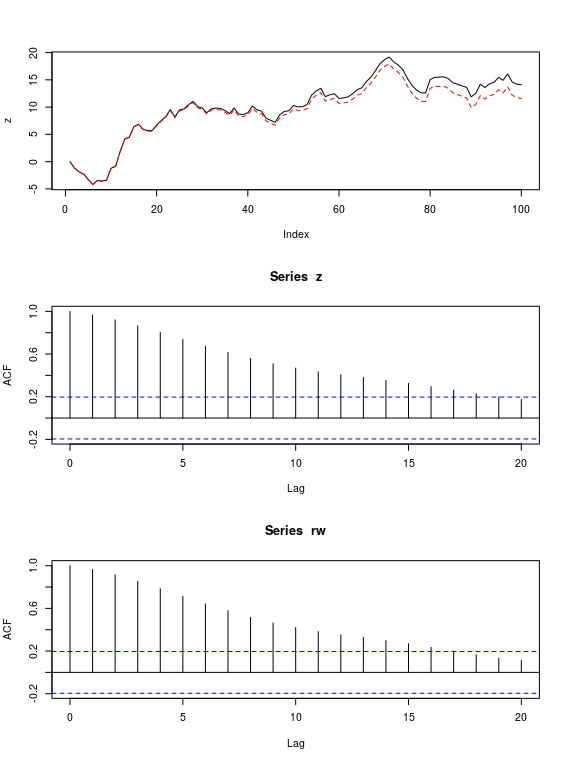
\includegraphics[width=1\textwidth]{fig1.png}
\end{figure}

\ck (재질문) 이 그림에서 젤 위의 빨간선은 랜덤워크이고 검은선은 트렌트를 포함한 AR(1)모형임. 그래서 빨간선은 비정상. 검은선은 정상임. 그리고 두번째 세번째는 각각의 ACF임. 구분가능함? 

\ck (답변) ... 


\ck (재질문) 사실 저런 경우는 ACF 찍어도 모르는거아님? 그리고 막말로 ACF 찍어도 잘 모르는거 많자나? ACF찍어서 알아내란 소리는 거의 ACF찍어서 ARMA($p$,$q$)에서 $p$, $q$를 결정할 수 있는 논리랑 동급으로 무책임한 말 아님? 

\ck (재질문) 막말로 확률적 추세 결정적 추세 구분못하자나? 아니 다 구분할 수 있었으면 머 분석자의 감이 필요하니.. 사전지식을 활용하라느니 구차하게 그런 말을 왜함? ACF로 구분하기 힘드니까 이것저것 여러개 방법 제시하는거 아님? 

\ck (답변) ... 

\ck (재질문) 그러니까 확률적 추세 결정적 추세 딱 구분하는 방법이 뭐냐고요. 

\ck (답변) ... 

\ck (재질문) 그냥 두번 차분할껀데 할말 있어요? 

\ck (답변) ... 

\ck (규빈) 구분이 쉽지 않다는걸 인정하고 특정예제의 경우 과대차분이 큰 문제가 안될수도 있다는것도 동의함. 다만 구분을 할 수 있으면 하는것이 좋다고 생각함. 

\ck (규빈) 때로는 결정적 추세와 비결정적 추세를 구분하는 일이 의사결정을 뒤흔들만한 중대한 일이 될수도 있음. 

\ck (규빈) 최소한 제시한 예제에서 이건 결정적 추세보다 확률적 추세인것 처럼 보인다. 라는 주장자체는 할 줄 알아야함. (그것이 틀린주장이라고 하더라도)

\ck (규빈) 랜덤워크와 회귀모형의 근본적 차이는 추세가 미래에 지속될것이라 믿느냐임. 이러한 차이를 모르는사람이 있다고 가정하자. 이 사람이 제시한 그림의 $t=15$쯤에서 시계열을 관측했다고 가정하자. 이 사람은 이렇게 생각할 것이다. 

\one 아 이거 기세가 뭔가 오르는 느낌이 드는데? 

\ck (규빈) 하지만 당신이 이 모형을 랜덤워크라고 판단했으면 이런 기세따위는 없음을 알고 있을 것이다. 

\ck (규빈) 랜덤워크라는 개념이 없는사람이 이 모형을 계속 관찰하였다고 하자. $t=40$까지 관측하였다. 이 사람은 이렇게 생각할 것이다. 

\two 이제는 사야겠다. 이건 오르는 주식이야. 

\ck (규빈) 랜덤워크는 사실을 알고 있는사람이라면? 역시 안산다. 

\end{document}
